\documentclass[11pt]{beamer}
\usepackage[english]{babel}
\usetheme{madrid}

%%%%%%%%%%% Instructions %%%%%%%%%%%%%
% 1. You must not make any changes to the preamble of this file.
% 2. Use this template for the beamer question in exam.
%%%%%%%%%%%%%%%%%%%%%%%%%%%%%%


\begin{document}
\title{Two Interesting Curves} 
\author{Student ID} 
\date{\today}
%%%%%%%%%%%%

\begin{frame} \label{front} % Slide 1
\titlepage


\end{frame}
%%%%%%%%%%%%
\begin{frame} \frametitle{Table of Contents}\label{ToC} % Slide 2

\tableofcontents

\end{frame}
%%%%%%%%%%%%
\section{TwoCurves}
\begin{frame} \frametitle{Two Curves} \label{TC}% Slide 3
\begin{columns}
\column<1->{0.5\textwidth}
$f(x)=(\sin(x)+\cos(x))\cdot (\cos(x)-2)$\\
$g(x)=e^{2\sin(x)}$

\column<2->{0.5\textwidth}
\begin{figure}
\centering
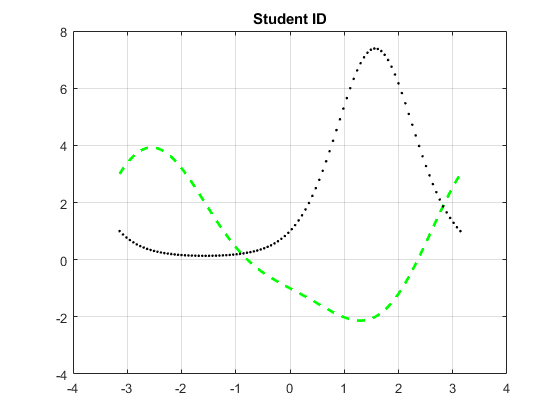
\includegraphics[scale=0.45]{twoPlots}
\caption{Two Plots}
\end{figure}
\end{columns}

\end{frame}
%%%%%%%%%%%%
\section{Observation}
\begin{frame} \frametitle{Observation}\label{Obs}% Slide 4
\begin{block}{Points of Intersection}<1->
There are 2 (two) points of intersection.
\end{block}

\begin{block}{Question}<2->
The points of intersection can be found by solving $f(x)=g(x)$.
\end{block}

\begin{block}{Min/Max}<3->
Any reasonable statement about min/max.
\end{block}

\end{frame}
%%%%%%%%%%%%
\section{Summary}
\begin{frame} \frametitle{Summary} % Slide 5
\hyperlink{Obs}{\beamergotobutton{Back to Observation}}\\
\hyperlink{TC}{\beamergotobutton{Back to Two Curves}}\\
\hyperlink{TOC}{\beamergotobutton{Back to Contents}}\\
\hyperlink{front}{\beamergotobutton{Back to Title}}

\end{frame}


\end{document}